\chapter{Implementação}

A solução encontra-se dividida em vários projetos de bibliotecas, aplicações de consola e uma aplicação WinForm. 

\section{Central Manager} \label{seccentralmanager}

Para ser implementado o servidor central, foi necessário definir a interface ICentralManager, apresentada na figura \ref{icentralmanager}.\\ 

\begin{figure}[h]
	\makebox[\textwidth][c]{
		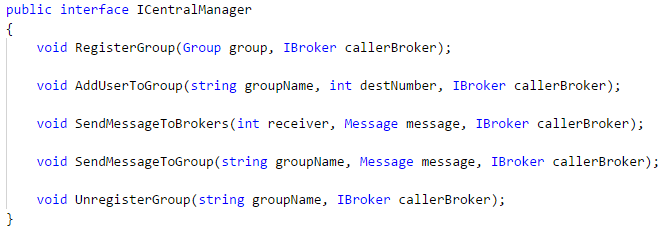
\includegraphics[width=1.0\textwidth]{./figures/icentralmanager}
	}
	\caption{Interface ICentralManager}
	\label{icentralmanager}
\end{figure}

O \textit{central manager} conhece todos os servidores regionais existentes, pois é injetado no construtor uma lista com todos os \textit{proxies} dos servidores regionais desse sistema. Desta forma, o \textit{central manager} é \textit{stateless} visto que não armazena mais nenhuma informação.\\

Para a implementação do \textit{central manager}, foi usado o padrão \textit{singleton}. O padrão \textit{singleton} adequa-se melhor às necessidades, pois assume-se que o servidor central estará sempre a receber e a enviar pedidos. Desta forma o padrão \textit{single call} teria muito maior \textit{overhead} em relação ao \textit{singleton} pois teria de estar sempre a criar novas instâncias para responder a cada pedido, sendo que não se sabe o número de pedidos de antemão.\\

De modo a que não é possível determinar o uso deste sistema distribuído, não existe forma de saber se é usado com bastante regularidade e com espaçamento no intervalo de tempo entre as mensagens; No pior dos casos tem o objeto em memória com tempo infinito e os pedidos nunca passam pelo \textit{manager}, e no melhor dos casos os pedidos são atendidos sempre pela mesma instância, sem esta estar a ocupar recursos em memória desnecessariamente.\\

O \textit{lease time} escolhido para a instância do \textit{central manager} foi zero, o que significa que o seu tempo de vida é infinito. Foi tomada esta decisão porque a implementação de \textit{Central Manager} não tem nenhum construtor sem parâmetros, pelo que o CLR não conseguiria criar uma nova instância, caso esta tenha sido apagada. O inconveniente desta solução é ter recursos ocupados sem haver necessidade de os ter, uma vez que esta instância pode não estar a servir pedidos. 

\section{Broker} \label{broker}

Para implementar o servidor regional, definiu-se duas interfaces. A interface para interação com o utilizador é IBrokerService, apresentada na figura \ref{ibrokerservice}. 

\begin{figure}[h]
	\makebox[\textwidth][c]{
		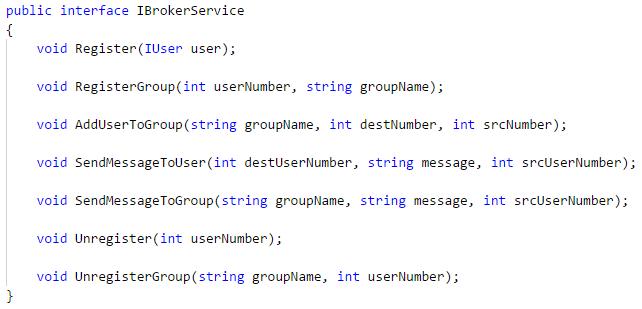
\includegraphics[width=1.0\textwidth]{./figures/ibrokerservice}
	}
	\caption{Interface IBrokerService}
	\label{ibrokerservice}
\end{figure}

A interface para a interação com o \textit{central manager} é IBrokerClient, apresentada na figura \ref{ibrokerclient}.

\begin{figure}[h]
	\makebox[\textwidth][c]{
		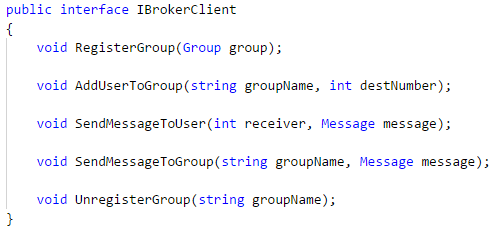
\includegraphics[width=0.9\textwidth]{./figures/ibrokerclient}
	}
	\caption{Interface IBrokerClient}
	\label{ibrokerclient}
\end{figure}

O \textit{broker} mantém informação dos utilizadores registados nessa região e dos grupos existentes em todas as regiões. Desta forma, o \textit{broker} é \textit{stateful}.\\

Para a implementação do \textit{broker} foi usado o padrão \textit{singleton}. Foi usado este padrão, pois existe a necessidade de manter estado. Se fosse usado o padrão \textit{single call}, tal não era permitido porque seria criado uma instância por cada pedido, impossibilitando a agregação de informação.\\

O \textit{lease time} escolhido foi zero, o que significa que este terá um tempo de vida infinito. Isto porque devido à necessidade de manter estado, se fosse chamado o desconstrutor da instância, perder-se-ia toda a informação sobre os utilizadores e grupos.\\

\section{User} \label{user}

Para implementar o cliente, definiu-se a interface apresentada na figura \ref{iuser}.

\begin{figure}[h]
	\makebox[\textwidth][c]{
		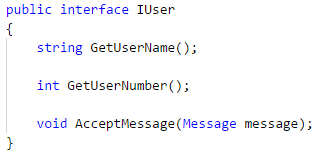
\includegraphics[width=0.6\textwidth]{./figures/iuser}
	}
	\caption{Interface IUser}
	\label{iuser}
\end{figure}

A implementação da interface também extende de \textit{MarshalByRefObject} porque a referência do objeto será enviado para um \textit{broker}.\\ 

\section{Controlo de Concorrência} \label{concorrencia}

Tanto o \textit{central manager} como o \textit{broker} seguem o padrão \textit{singleton}, como descrito anteriormente, e por essa razão o CLR do .NET irá atender os diferentes pedidos em diferentes \textit{threads}. Como as \textit{threads} irão aceder à mesma instância, é necessário garantir controlo de concorrência. Para garantir o acesso concorrente ao estado dessas instâncias, foi usado a biblioteca \textit{Concurrent} do .NET.\\

\section{Ficheiros de Configuração} \label{configuracao}

De forma a não comprometer o código com os URLs, protocolos, implementações e canais, foi usado ficheiros de configuração. 
Para poder ter vários URLs para o mesmo tipo, foi usada a \textit{tag appSettings}. Desta forma, é possível haver vários URIs para o mesmo tipo. Cada URI está associado a um \textit{broker}. O \textit{type} e o \textit{assembly} são duas entradas na \textit{tag} usadas para construir instâncias da classe \textit{WellKnownClientTypeEntry}. Assim, tem-se definido estáticamente quais os \textit{brokers} existentes neste sistema.\\

O \textit{TypeFilterLevel} usado em todos os ficheiros é \textit{Full} porque todas as interações entre as partes recebem como argumento um objeto que estende de \textit{MarshalByRefObject}.